% appendix/questions/after.tex

\section{What Does ``After'' Mean?}
\label{sec:app:questions:What Does ``After'' Mean?}

``After'' is an intuitive, but surprisingly difficult concept.
An important non-intuitive issue is that code can be delayed at
any point for any amount of time.
Consider a producing and a consuming thread that communicate using
a global struct with a timestamp ``t'' and integer fields ``a'', ``b'',
and ``c''.
The producer loops recording the current time
(in seconds since 1970 in decimal),
then updating the values of ``a'', ``b'', and ``c'',
as shown in Figure~\ref{fig:app:questions:After Producer Function}.
The consumer code loops, also recording the current time, but also
copying the producer's timestamp along with the fields ``a'',
``b'', and ``c'', as shown in
Figure~\ref{fig:app:questions:After Consumer Function}.
At the end of the run, the consumer outputs a list of anomalous recordings,
e.g., where time has appeared to go backwards.

{ \scriptsize
\begin{verbbox}
  1 /* WARNING: BUGGY CODE. */
  2 void *producer(void *ignored)
  3 {
  4   int i = 0;
  5
  6   producer_ready = 1;
  7   while (!goflag)
  8     sched_yield();
  9   while (goflag) {
 10     ss.t = dgettimeofday();
 11     ss.a = ss.c + 1;
 12     ss.b = ss.a + 1;
 13     ss.c = ss.b + 1;
 14     i++;
 15   }
 16   printf("producer exiting: %d samples\n", i);
 17   producer_done = 1;
 18   return (NULL);
 19 }
\end{verbbox}
}
\begin{figure}[htbp]
\centering
\theverbbox
\caption{``After'' Producer Function}
\label{fig:app:questions:After Producer Function}
\end{figure}

{ \fontsize{6.5pt}{7.5pt}\selectfont
\begin{verbbox}
  1 /* WARNING: BUGGY CODE. */
  2 void *consumer(void *ignored)
  3 {
  4   struct snapshot_consumer curssc;
  5   int i = 0;
  6   int j = 0;
  7
  8   consumer_ready = 1;
  9   while (ss.t == 0.0) {
 10     sched_yield();
 11   }
 12   while (goflag) {
 13     curssc.tc = dgettimeofday();
 14     curssc.t = ss.t;
 15     curssc.a = ss.a;
 16     curssc.b = ss.b;
 17     curssc.c = ss.c;
 18     curssc.sequence = curseq;
 19     curssc.iserror = 0;
 20     if ((curssc.t > curssc.tc) ||
 21         modgreater(ssc[i].a, curssc.a) ||
 22         modgreater(ssc[i].b, curssc.b) ||
 23         modgreater(ssc[i].c, curssc.c) ||
 24         modgreater(curssc.a, ssc[i].a + maxdelta) ||
 25         modgreater(curssc.b, ssc[i].b + maxdelta) ||
 26         modgreater(curssc.c, ssc[i].c + maxdelta)) {
 27       i++;
 28       curssc.iserror = 1;
 29     } else if (ssc[i].iserror)
 30       i++;
 31     ssc[i] = curssc;
 32     curseq++;
 33     if (i + 1 >= NSNAPS)
 34       break;
 35   }
 36   printf("consumer exited, collected %d items of %d\n",
 37          i, curseq);
 38   if (ssc[0].iserror)
 39     printf("0/%d: %.6f %.6f (%.3f) %d %d %d\n",
 40            ssc[0].sequence, ssc[j].t, ssc[j].tc,
 41            (ssc[j].tc - ssc[j].t) * 1000000,
 42            ssc[j].a, ssc[j].b, ssc[j].c);
 43   for (j = 0; j <= i; j++)
 44     if (ssc[j].iserror)
 45       printf("%d: %.6f (%.3f) %d %d %d\n",
 46              ssc[j].sequence,
 47              ssc[j].t, (ssc[j].tc - ssc[j].t) * 1000000,
 48              ssc[j].a - ssc[j - 1].a,
 49              ssc[j].b - ssc[j - 1].b,
 50              ssc[j].c - ssc[j - 1].c);
 51   consumer_done = 1;
 52 }
\end{verbbox}
}
\begin{figure}[htbp]
\centering
\theverbbox
\caption{``After'' Consumer Function}
\label{fig:app:questions:After Consumer Function}
\end{figure}

\QuickQuiz{}
	What SMP coding errors can you see in these examples?
	See \path{time.c} for full code.
\QuickQuizAnswer{
	\begin{enumerate}
	\item	Missing barrier() or volatile on tight loops.
	\item	Missing Memory barriers on update side.
	\item	Lack of synchronization between producer and consumer.
	\end{enumerate}
} \QuickQuizEnd

One might intuitively expect that the difference between the producer
and consumer timestamps would be quite small, as it should not take
much time for the producer to record the timestamps or the values.
An excerpt of some sample output on a dual-core 1GHz x86 is shown in
Table~\ref{tab:app:questions:After Program Sample Output}.
Here, the ``seq'' column is the number of times through the loop,
the ``time'' column is the time of the anomaly in seconds, the ``delta''
column is the number of seconds the consumer's timestamp follows that
of the producer (where a negative value indicates that the consumer
has collected its timestamp before the producer did), and the
columns labelled ``a'', ``b'', and ``c'' show the amount that these
variables increased since the prior snapshot collected by the consumer.

\begin{table}[htbp]
\centering
\scriptsize
\begin{tabular}{rcrrrr}
seq    & time (seconds) & delta~    &  a &  b &  c \\
\hline
17563: & 1152396.251585 & ($-16.928$) & 27 & 27 & 27 \\
18004: & 1152396.252581 & ($-12.875$) & 24 & 24 & 24 \\
18163: & 1152396.252955 & ($-19.073$) & 18 & 18 & 18 \\
18765: & 1152396.254449 & ($-148.773$) & 216 & 216 & 216 \\
19863: & 1152396.256960 & ($-6.914$) & 18 & 18 & 18 \\
21644: & 1152396.260959 & ($-5.960$) & 18 & 18 & 18 \\
23408: & 1152396.264957 & ($-20.027$) & 15 & 15 & 15 \\
\end{tabular}
\caption{``After'' Program Sample Output}
\label{tab:app:questions:After Program Sample Output}
\end{table}

Why is time going backwards?
The number in parentheses is the difference in microseconds, with
a large number exceeding 10 microseconds, and one exceeding even
100 microseconds!
Please note that this CPU can potentially execute more than 100,000
instructions in that time.

One possible reason is given by the following sequence of events:
\begin{enumerate}
\item	Consumer obtains timestamp
	(Figure~\ref{fig:app:questions:After Consumer Function}, line~13).
\item	Consumer is preempted.
\item	An arbitrary amount of time passes.
\item	Producer obtains timestamp
	(Figure~\ref{fig:app:questions:After Producer Function}, line~10).
\item	Consumer starts running again, and picks up the producer's
	timestamp
	(Figure~\ref{fig:app:questions:After Consumer Function}, line~14).
\end{enumerate}

In this scenario, the producer's timestamp might be an arbitrary
amount of time after the consumer's timestamp.

How do you avoid agonizing over the meaning of ``after'' in your
SMP code?

Simply use SMP primitives as designed.

In this example, the easiest fix is to use locking, for example,
acquire a lock in the producer before line 10 in
Figure~\ref{fig:app:questions:After Producer Function} and in
the consumer before line~13 in
Figure~\ref{fig:app:questions:After Consumer Function}.
This lock must also be released after line~13 in
Figure~\ref{fig:app:questions:After Producer Function} and
after line 17 in
Figure~\ref{fig:app:questions:After Consumer Function}.
These locks cause the code segments in lines~10-13 of
Figure~\ref{fig:app:questions:After Producer Function} and in lines~13-17 of
Figure~\ref{fig:app:questions:After Consumer Function} to {\em exclude}
each other, in other words, to run atomically with respect to each other.
This is represented in
Figure~\ref{fig:app:questions:Effect of Locking on Snapshot Collection}:
the locking prevents any of the boxes of code from overlapping in time, so
that the consumer's timestamp must be collected after the prior
producer's timestamp.
The segments of code in each box in this figure are termed
``critical sections''; only one such critical section may be executing
at a given time.

\begin{figure}[htb]
\centering
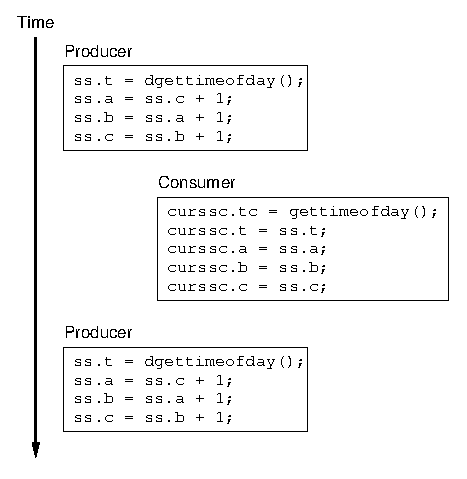
\includegraphics{appendix/questions/after}
\caption{Effect of Locking on Snapshot Collection}
\label{fig:app:questions:Effect of Locking on Snapshot Collection}
\end{figure}

This addition of locking results in output as shown in
Table~\ref{fig:app:questions:Locked After Program Sample Output}.
Here there are no instances of time going backwards, instead,
there are only cases with more than 1,000 counts difference between
consecutive reads by the consumer.

\begin{table}[htbp]
\centering
\scriptsize
\begin{tabular}{rcrrrr}
seq    & time (seconds) & delta~    &  a &  b &  c \\
\hline
58597:  & 1156521.556296 & (3.815) & 1485 & 1485 & 1485 \\
403927: & 1156523.446636 & (2.146) & 2583 & 2583 & 2583 \\
\end{tabular}
\caption{Locked ``After'' Program Sample Output}
\label{fig:app:questions:Locked After Program Sample Output}
\end{table}

\QuickQuiz{}
	How could there be such a large gap between successive
	consumer reads?
	See \path{timelocked.c} for full code.
\QuickQuizAnswer{
	\begin{enumerate}
	\item	The consumer might be preempted for long time periods.
	\item	A long-running interrupt might delay the consumer.
	\item	The producer might also be running on a faster CPU than is the
		consumer (for example, one of the CPUs might have had to
		decrease its
		clock frequency due to heat-dissipation or power-consumption
		constraints).
	\end{enumerate}
} \QuickQuizEnd

In summary, if you acquire an exclusive lock, you {\em know} that
anything you do while holding that lock will appear to happen after
anything done by any prior holder of that lock.
No need to worry about which CPU did or did not execute a memory
barrier, no need to worry about the CPU or compiler reordering
operations---life is simple.
Of course, the fact that this locking prevents these two pieces of
code from running concurrently might limit the program's ability
to gain increased performance on multiprocessors, possibly resulting
in a ``safe but slow'' situation.
Chapter~\ref{cha:Partitioning and Synchronization Design} describes ways of
gaining performance and scalability in many situations.

However, in most cases, if you find yourself worrying about what happens
before or after a given piece of code, you should take this as a hint to
make better use of the standard primitives.
Let these primitives do the worrying for you.
